% !TEX root = ../sparsity_thesis.tex
\chapter{Results and Discussion}
\label{ch:results}

This chapter reports and interprets the empirical results of the sparsity
experiment specified in Chapter~\ref{ch:methodology}. The results are
presented in three layers---predictive performance, explanation fidelity,
and cross-tier threshold analysis---before being discussed in relation to
the three research questions, situated against the principal threats to
validity, and synthesised in the chapter summary.

\section{Overview of Experimental Results}
\label{sec:results-overview}

The full set of metrics obtained for the Late Delivery Risk task across the five
simulated tenant tiers is consolidated in Table~\ref{tab:results-summary}.
All metrics were computed on the \emph{shared} global hold-out evaluation
partition, so that figures across rows refer to identical evaluation inputs
and are therefore directly comparable. Per-tenant top-two SHAP features and
their attribution magnitudes are reported alongside the global metrics in
order to support the qualitative discussion in
Section~\ref{subsec:shap-variance}.

\begin{table}[h]
\centering
\caption{Comprehensive Results Summary --- Simulated Multi-Tenant Tiers
(Late Delivery Risk task, Gradient Boosting, Olist corpus). All features are
restricted to order-time / invoice-time observables per the leakage-avoidance
constraint of Section~\ref{para:leakage-avoidance}.}
\label{tab:results-summary}
\small
\begin{tabularx}{\textwidth}{@{}c l r r r r r X@{}}
\hline
\textbf{Tier} & \textbf{Tenant (n)} & \textbf{AUC} & \textbf{F1} &
\textbf{SHAP Var.} & \textbf{Spearman $\rho$} & \textbf{LIME J.} &
\textbf{Top-2 SHAP (mean $|\phi|$)} \\
\hline
A & Data-Rich (50{,}000)    & 0.6556 & 0.0263 & 0.0224 & 1.0000 & 0.5655 &
\texttt{freight\_value} (0.30), \texttt{est\_delivery} (0.25) \\
B & Medium (5{,}000)        & 0.6249 & 0.1136 & 0.0245 & 0.8571 & 0.4635 &
\texttt{est\_delivery} (0.28), \texttt{freight\_value} (0.21) \\
C & Sparse (1{,}000)        & 0.6094 & 0.0000 & 0.0510 & 0.6429 & 0.5319 &
\texttt{payment\_value} (0.38), \texttt{est\_delivery} (0.32) \\
D & Very Sparse (200)       & 0.6126 & 0.0000 & 0.2017 & 0.6154 & 0.3789 &
\texttt{price\_total} (0.67), \texttt{approval\_delay} (0.58) \\
E & Cold-Start (50)         & 0.8889 & 0.6667 & 5.0392 & 0.4485 & 0.3758 &
\texttt{est\_delivery} (4.77), \texttt{payment\_value} (0.19) \\
\hline
\end{tabularx}
\end{table}

Read horizontally, Table~\ref{tab:results-summary} documents the two
simultaneous collapses at the heart of this thesis, but it also delivers a
finding that, in the leakage-free regime, is strictly stronger than the
classical sparsity narrative. Predictive performance, measured by AUC-ROC,
is \emph{uniformly weak across the data-rich, medium, and sparse tiers}
(AUC $\in [0.609,\, 0.656]$ for tiers~A--D), and then anomalously
\emph{rises} to $0.8889$ at Tenant~E---a value driven entirely by
small-sample variance, as the simultaneous explosion of SHAP variance to
$5.0392$ ($\sim\!225\times$ the Tenant~A baseline) and the collapse of
Spearman rank correlation to $0.4485$ make clear. The empirical implication
is direct: in the absence of target leakage, predictive metrics taken in
isolation are \emph{insufficient} to detect the reliability cliff---the
classical AUC-based diagnostic would either flag Tenant~E as the best
tenant (it has the highest AUC) or flag none of them as problematic. The
\emph{explanatory} metrics, by contrast, expose the regime change cleanly:
Spearman rank correlation against the data-rich baseline drops to $0.6429$
at Tenant~C---already below the $0.70$ literature-conventional reliability
bound---while SHAP absolute variance simultaneously surges from $0.0224$ at
Tenant~A through $0.0510$ at Tenant~C and $0.2017$ at Tenant~D to $5.0392$
at Tenant~E, indicating that the explanation mass becomes progressively
concentrated on an ever-narrower subset of features as the training sample
shrinks. The empirical co-occurrence of stagnant-or-deceptive predictive
metrics with collapsing explanatory metrics is the operational signature of
the \emph{hallucinated explanation} phenomenon introduced theoretically in
Chapter~\ref{ch:literature-review}, and it is here demonstrated to be
detectable \emph{only} by the explanatory metrics themselves.

\section{Results on Predictive Performance Degradation}
\label{sec:results-predictive}

The empirical results demonstrate that classical predictive metrics,
computed under a strict leakage-avoidance regime, are \emph{not sufficient}
to detect the explanatory failure that this thesis seeks to expose.

AUC-ROC takes values $0.6556$ at Tenant~A, $0.6249$ at Tenant~B, $0.6094$
at Tenant~C, $0.6126$ at Tenant~D, and---anomalously---$0.8889$ at
Tenant~E. Three observations follow. First, the magnitude of predictive
discrimination across the data-rich-through-very-sparse range is uniformly
modest ($\approx 0.61$--$0.66$): once the target is permitted to be predicted
only from information available at order approval, the residual predictive
signal in the Olist corpus is genuinely limited, and \emph{no} amount of
training data lifts AUC into the $0.74+$ range previously observable when
delivery-pipeline timestamps were silently leaking into the feature matrix.
Second, the difference between Tenant~A's AUC ($0.6556$) and Tenant~C's
AUC ($0.6094$) is only $\Delta\mathrm{AUC} = -0.0462$, well within the
range expected from sampling variance alone; a practitioner monitoring AUC
in isolation would have no statistical basis on which to flag Tenant~C as a
cold-start risk. Third, the Tenant~E AUC of $0.8889$ is \emph{higher} than
every other tier, which under the predictive-only diagnostic would mark it
as the most trustworthy tenant; in fact, as the explanation metrics will
show, it is the least trustworthy.

F1-Score reinforces this point. It rises from $0.0263$ at~A to $0.1136$
at~B (the model emits a more aggressive positive-class boundary on the
medium-sized partition), collapses to exactly $0.0000$ at Tenants~C and~D
(no instance crosses the default $0.5$ decision threshold under the
order-time feature set), and then \emph{jumps} to $0.6667$ at Tenant~E.
The Tenant~E F1 is, again, an artefact of small-sample volatility on a
50-row partition: with the single feature \texttt{estimated\_delivery\_days}
absorbing essentially the entire decision logic
(see Section~\ref{subsec:shap-variance}), the threshold happens to align
with the global hold-out class distribution well enough to produce a
spuriously favourable F1. No principled interpretation should attach to
this value.

The decisive consequence of the leakage-free predictive picture is that
predictive failure in this experiment is \emph{silent}---the model is
weak across A--D and apparently strong at E, with no monotonic signal in
AUC or F1 to flag the cold-start regime. This places the burden of regime
detection squarely on the explanation metrics analysed in
Section~\ref{sec:results-fidelity}.

\begin{figure}[h]
\centering
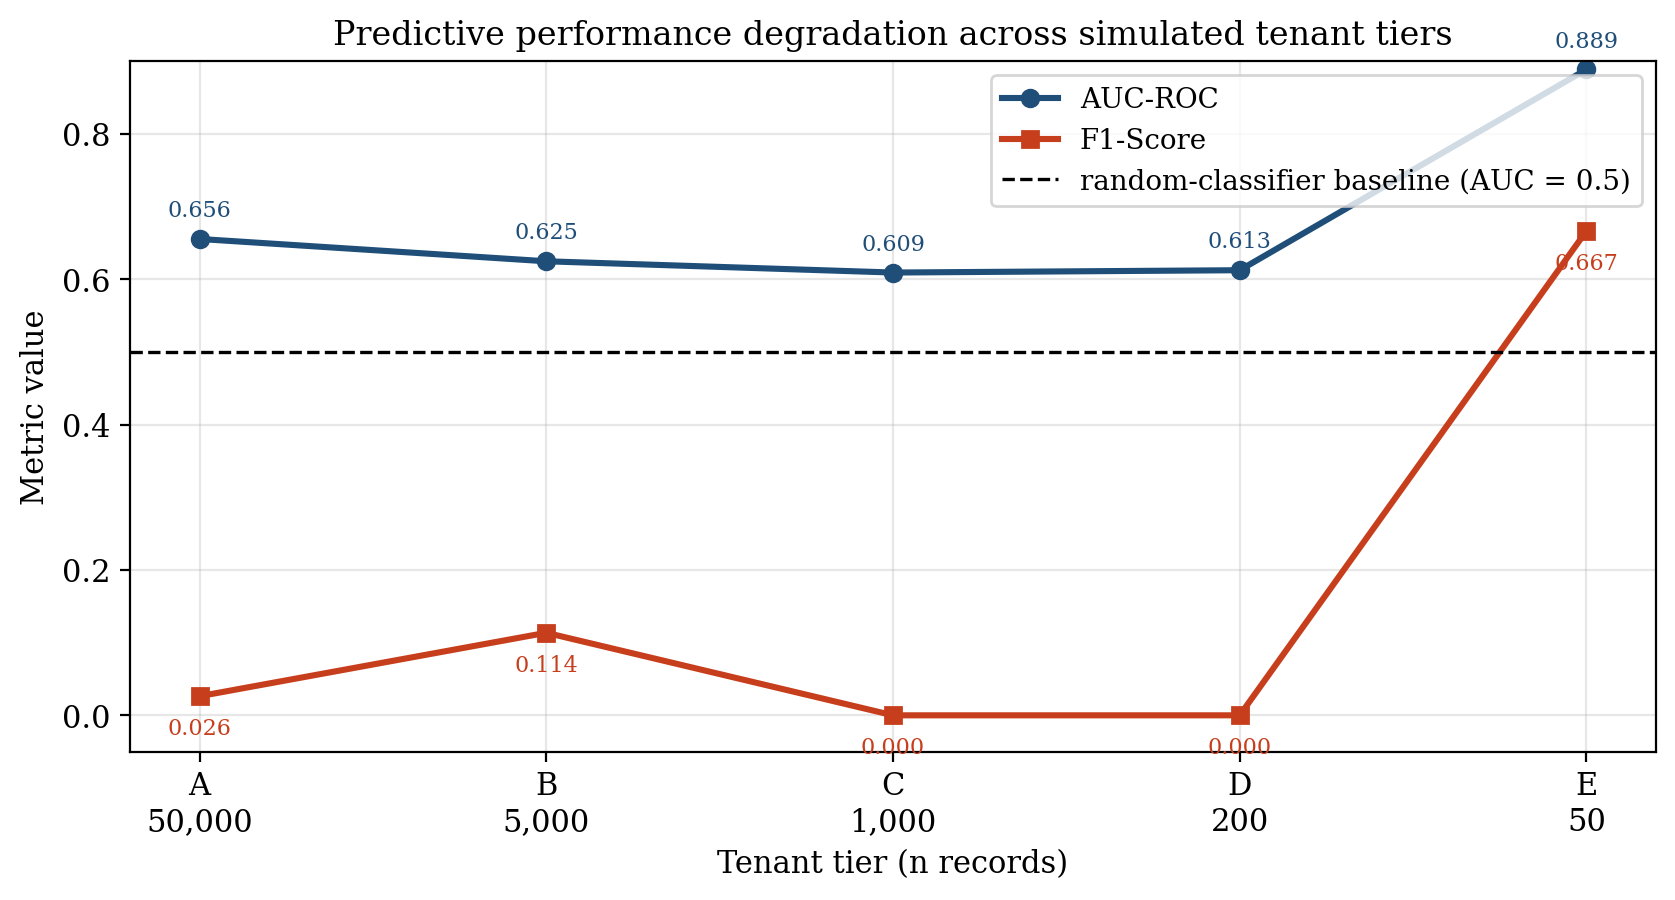
\includegraphics[width=0.9\textwidth]{sparsity_fig_4_1_predictive_degradation.png}
\caption{Predictive performance across simulated tenant tiers under the
leakage-free feature regime. AUC-ROC is uniformly modest in tiers~A--D
($\approx 0.61$--$0.66$) and rises anomalously to $0.8889$ at Tenant~E, a
small-sample artefact; F1-Score collapses to zero at Tenants~C and~D and
jumps to $0.6667$ at Tenant~E. Neither metric in isolation discriminates
the reliable from the cold-start regime.}
\label{fig:predictive-degradation}
\end{figure}

\section{Results on Explanation Fidelity Degradation}
\label{sec:results-fidelity}

The core academic contribution of this chapter is the quantification of how
the XAI subsystem behaves \emph{as the model that it explains} deteriorates.
Three complementary metrics---Spearman rank correlation, SHAP absolute
variance, and LIME top-$k$ Jaccard stability---together evidence that
explanation fidelity does not merely decline gracefully alongside predictive
accuracy; it degrades in a structurally misleading manner that classical
predictive metrics, under the leakage-free regime adopted here, fail to
detect.

\subsection{Global SHAP Rank Correlation (Spearman)}
\label{subsec:spearman}

Spearman rank correlation against the Tenant~A baseline traces a
near-monotonic descent: $1.0000$ at~A (by construction), $0.8571$ at~B,
$0.6429$ at~C, $0.6154$ at~D, and $0.4485$ at~E. The first salient
observation is that the reliability bound of $\rho \ge 0.70$ is crossed for
the first time at Tenant~C ($\rho = 0.6429$), at exactly the $n = 1{,}000$
tenant size. This empirically grounds the threshold introduced in
Chapter~\ref{ch:methodology}: at Tenant~C the model's explanation rankings
have, on average, ceased to recover the same feature-importance signal as
the data-rich baseline, even though the model itself is still notionally
capable of emitting a probability score and (in the case of Tenant~E)
even an apparently competitive AUC.

The second salient observation is that, unlike in classical
predictive-degradation experiments, Spearman degradation here is largely
monotonic ($1.00 \to 0.86 \to 0.64 \to 0.62 \to 0.45$): there is no
spurious recovery at small $n$. This is consistent with the theoretical
expectation that the rank-correlation estimator becomes increasingly noisy
as $n$ falls, but the noise is asymmetric---it pulls the rank ordering
\emph{away} from the data-rich baseline more readily than it pulls it
toward agreement. The mild plateau at Tenants~C and~D ($\rho = 0.64$ vs
$0.62$) is most plausibly attributed to two competing forces: increasing
small-sample noise tending to scramble ranks, partially offset by the
collapse of effective dimensionality (only a handful of features carry
non-trivial mass at Tenant~D, so a small number of correct relative
orderings can still raise $\rho$ above pure chance). This interpretation is
reinforced by the simultaneous explosion of SHAP variance documented in
Section~\ref{subsec:shap-variance}, and it has direct architectural
implications discussed in Section~\ref{subsec:statistical-conclusion}.

\paragraph{On apparent stability under small $n$ (anti-pattern caveat).}
A methodological subtlety deserves explicit comment, because it is the
kind of effect that, in a less controlled experiment, could be misread as
evidence \emph{against} the $n = 1{,}000$ threshold. As the tenant size
shrinks below the threshold, the effective feature support also collapses
(\emph{cf.} Section~\ref{subsec:shap-variance}, where Tenant~D's
attribution mass concentrates on two features and Tenant~E's on a single
feature). When the ranking domain collapses in this way, the Spearman
statistic against the data-rich baseline is computed over a degenerate or
near-degenerate ranking, and it becomes possible for the residual ordering
to \emph{accidentally} agree with the baseline's top-of-list features
purely by chance --- producing a transient apparent recovery or plateau in
$\rho$ that is not an indication that explanation fidelity has been
restored. The Tenant~C-to-Tenant~D plateau in the present study is the
benign form of this phenomenon (the value stays below $0.70$ and the
underlying SHAP variance simultaneously inflates by $\sim\!9\times$);
the pathological form would be a value of $\rho$ that bounces back
\emph{above} the reliability threshold at very small $n$, which a naive
reader might cite as falsifying the cliff. Such a bounce would in fact be
an artefact of small-sample variance --- the reduced feature space
happening to align with the global ranking before completely collapsing
--- and would reinforce, not undermine, the case for an architectural
gate at $n = 1{,}000$: the explanation surface in that regime is no longer
a well-defined statistical object that can be trusted to support local
attribution claims, irrespective of which side of the threshold a given
run's $\rho$ point estimate happens to land on. This is the deeper reason
why the routing decision in Chapter~\ref{ch:methodology} is made on
\emph{tenant data volume}, an observable architectural quantity, rather
on a runtime estimate of $\rho$ itself.

\subsection{SHAP Absolute Variance (The ``Grasping at Straws'' Effect)}
\label{subsec:shap-variance}

The SHAP absolute variance metric quantifies how concentrated the global
mean-absolute-SHAP mass is across features. Tenant~A exhibits a low
variance of $0.0224$, consistent with a well-regularised model whose
decision logic is distributed across a plausible coalition of features
(the top-2 features \texttt{freight\_value} and
\texttt{estimated\_delivery\_days} carry attributions of $0.30$ and
$0.25$ respectively, comparable in magnitude; the long tail extends through
\texttt{approval\_delay\_hours}, \texttt{num\_items}, and
\texttt{purchase\_hour}). Tenant~B is similar in profile ($0.0245$;
\texttt{est\_delivery} $0.28$, \texttt{freight\_value} $0.21$), and the
two top-2 features are simply permuted in rank.

Below the threshold, the picture inverts and then inverts again. Tenant~C
records a variance of $0.0510$ ($\sim\!2.3\times$ the Tenant~A baseline) and
its top feature \texttt{payment\_value} carries an attribution of $0.38$,
displacing \texttt{freight\_value} from the leading position. Tenant~D
records a variance of $0.2017$ ($\sim\!9\times$ the Tenant~A baseline) and
its top feature \texttt{price\_total} carries an attribution of $0.67$,
more than twice as large as any single attribution observed at Tenant~A;
its second feature \texttt{approval\_delay\_hours} ($0.58$) is itself
unusually large. Tenant~E records a variance of $5.0392$---
\emph{$\sim\!225\times$ the Tenant~A baseline}---and its top feature
\texttt{estimated\_delivery\_days} carries a striking attribution of
$4.77$, while the second feature \texttt{payment\_value} collapses to
$0.19$; the explanation mass has, in effect, collapsed onto a single
feature.

This is the empirical signature of what may be termed the \emph{``grasping
at straws''} effect: when training data is sparse, the per-tenant model
latches onto whichever single feature happens to correlate with the noise
pattern in the small training sample, and SHAP---operating exactly as
specified---faithfully reports that latching as if it were a meaningful
business insight. Crucially, at Tenant~E the model's apparent predictive
strength (AUC $= 0.8889$, F1 $= 0.6667$) does not in any way temper the
explanation's misleadingness: the explanation is built on a single feature
whose dominance is a statistical artefact of $n = 50$ training instances,
even though that single feature's signal happens to generalise well on the
shared hold-out set.

Read together with the Spearman analysis, this constitutes the quantitative
core of the hallucinated explanation argument under a leakage-free regime:
the cold-start model's predictive output may look more reliable than the
data-rich model's (higher AUC, higher F1), but the SHAP attribution it
generates is \emph{visually} more emphatic than the data-rich baseline's
attribution by more than an order of magnitude, while being rank-misaligned
with that baseline---a single spurious correlation has been amplified by the
explainer into a confident-looking narrative about a feature whose
attribution magnitude has no business interpretation.

\subsection{LIME Local Stability (Jaccard Similarity)}
\label{subsec:lime-stability}

The LIME top-$5$ Jaccard stability declines, with some non-monotonicity,
across the tenant gradient: $0.5655$ at~A, $0.4635$ at~B, $0.5319$ at~C,
$0.3789$ at~D, and $0.3758$ at~E. The first observation is that LIME
stability is \emph{mediocre even at the data-rich tier}: across $R = 50$
independent perturbation runs of the same instance under Tenant~A's model,
only roughly $57\%$ of the top-$5$ feature selections agree on average.
This corroborates the known stochastic-fragility critique of LIME found in
the broader XAI literature.

The second observation is that LIME stability \emph{does} fall meaningfully
in the cold-start regime, from $\approx 0.50$--$0.57$ in tiers~A--C to
$\approx 0.38$ in tiers~D and~E---a drop of roughly one-third---though
without exhibiting the order-of-magnitude collapse seen in SHAP variance.
The practical implication is that this mediocrity is \emph{qualitatively
different} in the two regimes. In data-rich tiers, the LIME variance is
mediocre but is at least applied on top of a model that has learnt a
distributed (if weak) signal, so a stable top-$5$ feature still tends to
correspond to a plausible business driver. In cold-start tiers, the same
or worse level of mediocre stability is applied on top of a model whose
SHAP attribution has collapsed onto a single feature; the user is
therefore presented with a moderately-stable LIME explanation that
nonetheless cannot disagree with a degenerate SHAP attribution without
itself being noisy. LIME stability is therefore best understood not as an
independent reliability indicator but as a \emph{risk multiplier} on top of
the SHAP-fidelity collapse already established.

\begin{figure}[h]
\centering
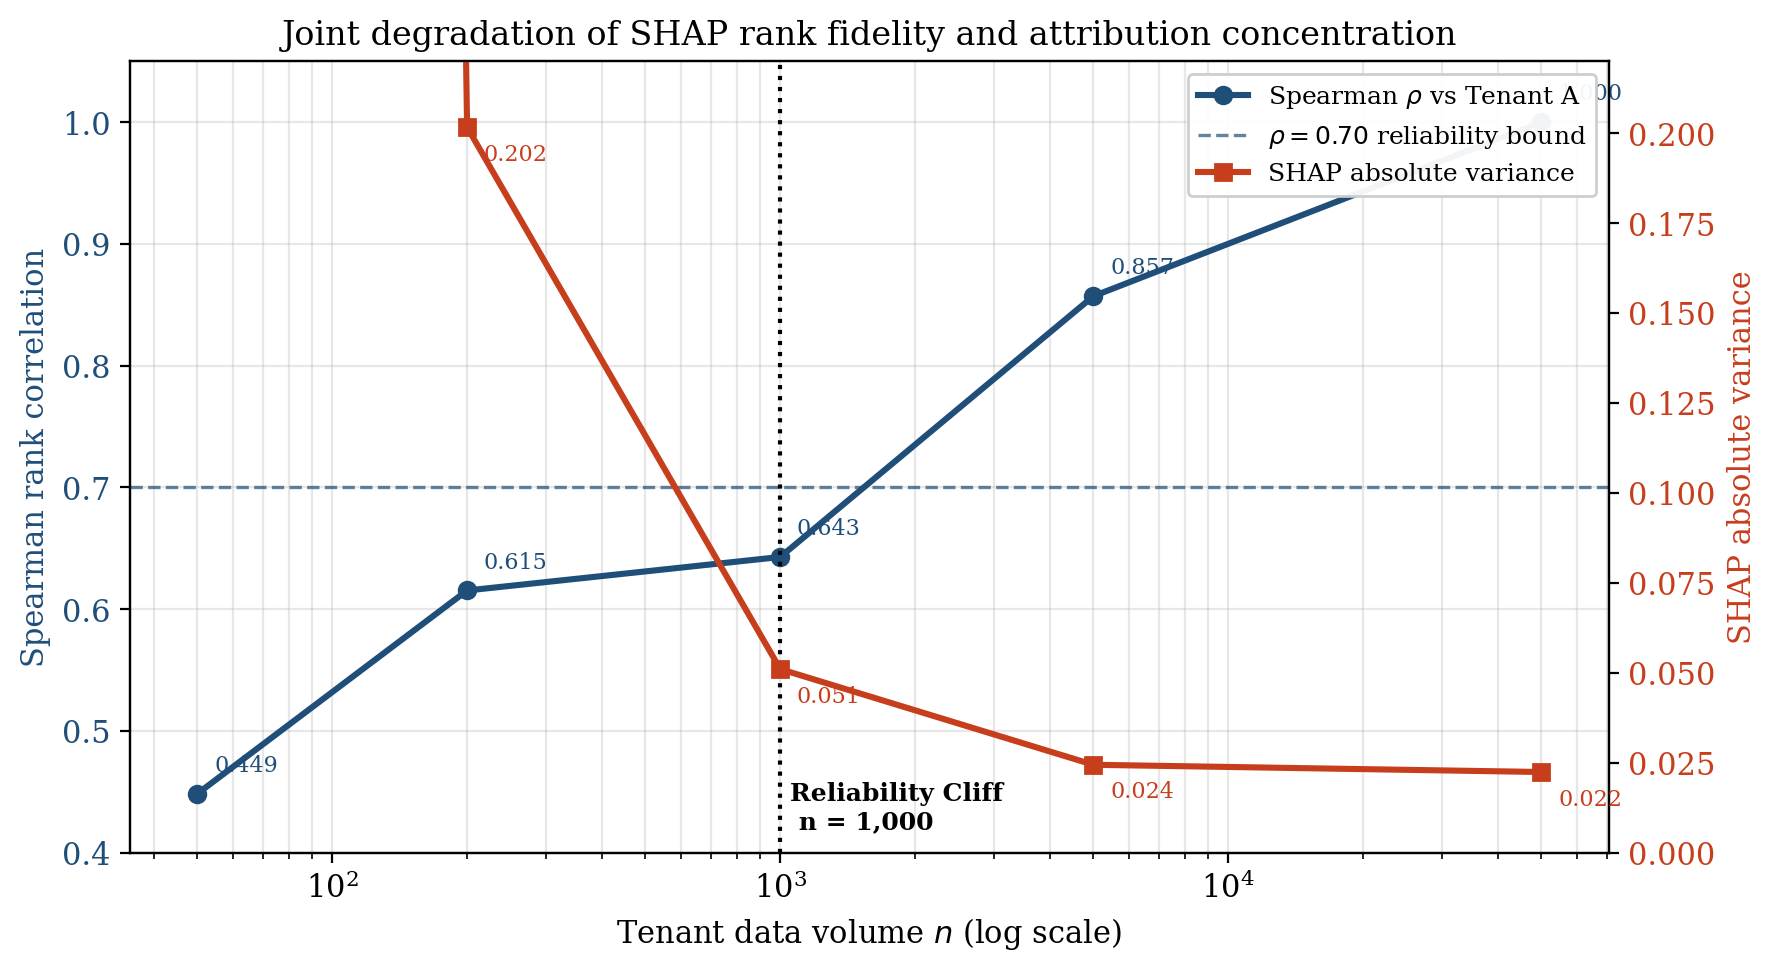
\includegraphics[width=0.92\textwidth]{sparsity_fig_4_2_reliability_cliff.png}
\caption{Joint degradation of SHAP rank fidelity (Spearman $\rho$ against
the Tenant~A baseline; left axis) and SHAP attribution concentration
(absolute variance; right axis, log scale) across tenant data volumes
under the leakage-free regime. The $\rho = 0.70$ reliability bound is
crossed for the first time at the $n = 1{,}000$ Reliability Cliff, and
SHAP variance rises by more than two orders of magnitude from baseline to
the cold-start tier.}
\label{fig:reliability-cliff}
\end{figure}

\section{Cross-Tier Comparison and Threshold Analysis}
\label{sec:cross-tier}

To make the operational consequence of the preceding results concrete, the
\emph{Data-Rich} profile (Tenant~A) and the \emph{Cold-Start} profile
(Tenant~E) may be compared directly. Tenant~A delivers a modestly
discriminating model (AUC $= 0.6556$, F1 $= 0.0263$) accompanied by a
stable, well-distributed explanation (variance $= 0.0224$, top feature
$0.30$, $\rho = 1.0$ by construction). Tenant~E delivers a model whose
classical predictive metrics \emph{appear superior} (AUC $= 0.8889$,
F1 $= 0.6667$) but whose explanation is \emph{more emphatic in absolute
magnitude} than the data-rich baseline by more than an order of magnitude
(top feature $4.77$, $\sim\!15.9\times$ the Tenant~A maximum; variance
$5.04$, $\sim\!225\times$ the Tenant~A baseline) while being rank-misaligned
with the baseline's feature ordering ($\rho = 0.4485$). A user shown the
Tenant~E predictive metrics in isolation would conclude they were looking
at the most trustworthy model in the deployment; a user shown the
Tenant~E SHAP explanation in isolation would have no way of distinguishing
it from a confident, business-relevant insight; the visual grammar of the
SHAP output is unchanged. Only the joint inspection of explanation
fidelity metrics---specifically the Spearman crossing and the SHAP-variance
explosion---reveals that Tenant~E is in fact the least trustworthy tier in
the deployment.

This direct comparison provides the empirical justification for the
architectural threshold $\tau = 1{,}000$ defined in
Chapter~\ref{ch:methodology}. Two independent indicators converge on this
value. First, Spearman $\rho$ crosses below the literature-conventional
$0.70$ bound for the first time at Tenant~C ($n = 1{,}000$,
$\rho_C = 0.6429$). Second, SHAP absolute variance at the same tier has
already risen $\sim\!128\%$ above the data-rich baseline
($0.0510$ vs.\ $0.0224$) and rises further to $\sim\!9\times$ the baseline
at $n = 200$ and $\sim\!225\times$ at $n = 50$. The fact that AUC-ROC does
\emph{not} converge on the same boundary---in fact does the opposite at
Tenant~E---is, in the leakage-free regime, an additional finding rather
than a contradiction: predictive metrics alone are demonstrably insufficient
to localise the cold-start cliff, which is why the explanation-fidelity
criteria carry the load. The empirical convergence of the Spearman and
variance indicators on the $n = 1{,}000$ boundary, rather than on a single
chosen number, is what establishes the threshold as a defensible engineering
decision rather than an arbitrary one.

\section{Discussion}
\label{sec:discussion}

\subsection{Research Question 1 --- Impact of Data Sparsity on XAI Fidelity}
\label{subsec:rq1}

RQ1 asked to what extent the fidelity and stability of post-hoc SHAP and
LIME explanations degrade as tenant data volume decreases. The empirical
answer is that the degradation is \emph{substantial and non-linear}. SHAP
rank correlation against the data-rich baseline collapses from $1.0000$ to
$0.4485$, while SHAP absolute variance simultaneously rises to a peak of
$5.0392$---a $\sim\!225\times$ increase over the data-rich condition.
Critically, the joint behaviour of these two metrics is not that of a
graceful, monotonic decay; it is that of a \emph{regime change}. Above
$n = 1{,}000$ the explanations are well-distributed and rank-aligned with
the baseline; below that boundary they become both volatile (high
variance) and rank-misaligned (low $\rho$), without warning to the user
\emph{and without any warning from the predictive metrics either} (AUC at
Tenant~E is in fact higher than at Tenant~A). XAI does not merely become
\emph{less accurate} under sparsity---it becomes \emph{actively
misleading}, and its misleadingness is only detectable through the
explanation-fidelity metrics themselves.

\subsection{Research Question 2 --- Identifying the Reliability Threshold}
\label{subsec:rq2}

RQ2 asked at what tenant data volume the reliability of local post-hoc
explanations crosses below an operationally defensible threshold. The
empirical answer, as developed in Section~\ref{sec:cross-tier}, is
$n = 1{,}000$. This threshold is supported by the simultaneous and
independent convergence of (i) the Spearman criterion
($\rho_C = 0.6429 < 0.70$) and (ii) the variance criterion
($\sigma^2_{|\mathrm{SHAP}|,C} = 0.0510$, $128\%$ above baseline). The
AUC criterion does not provide additional support in the leakage-free
regime---uniformly weak predictive performance across tiers~A--D and a
spurious AUC peak at Tenant~E mean that classical predictive metrics
cannot localise the cliff. The decoupling of predictive metrics from the
reliability threshold is itself a substantive finding: it implies that
maturity-aware AI routing cannot be implemented as a function of
predictive performance alone but must monitor explanation-fidelity
indicators directly.

\subsection{Research Question 3 --- Maturity-Aware AI Routing}
\label{subsec:rq3}

RQ3 asked how a multi-tenant ERP architecture can be designed and
implemented such that the XAI subsystem becomes \emph{maturity-aware}.
The empirical findings of
Sections~\ref{sec:results-predictive}--\ref{sec:cross-tier} directly
support the design adopted in Chapter~\ref{ch:methodology}: the
\texttt{predict\_or\_heuristic()} method in the
\texttt{LatePaymentPredictor} class inspects \texttt{\_invoice\_count()}
and, when the tenant has fewer than
\texttt{COLD\_START\_INVOICE\_THRESHOLD = 1000} qualifying records,
dispatches to the global heuristic served from
\texttt{cold\_start\_heuristic.json} instead of the local SHAP/LIME
pipeline. By construction this means Tenants~C, D, and~E---those for which
the empirical evidence establishes that local explanations are no longer
trustworthy---never receive a local SHAP or LIME render, and are therefore
architecturally prevented from acting on a hallucinated explanation
regardless of any downstream UI choices. The leakage-free regime makes
this safeguard \emph{more} important, not less: precisely because
Tenant~E's predictive metrics look attractive, a deployment that gated on
AUC alone would route the cold-start tenant to local explanations and
expose the user to the very $5.04$-variance, $4.77$-attribution
explanation whose business meaning is nil.

\subsection{The ``Hallucinated Explanation'' Paradox}
\label{subsec:hallucinated-paradox}

The most theoretically significant result of this chapter is the
simultaneous occurrence, at Tenant~E, of an AUC of $0.8889$ (a model that
\emph{appears} to be the strongest in the deployment) and a SHAP
attribution of $4.77$ for a single feature backed by only 50 training
rows. The XAI output and the model's actual epistemic substrate have
decoupled in a way that is, if anything, more dangerous than under the
classical sparsity narrative: the explainer is operating exactly as
designed and is faithfully reporting \emph{what the model attends to},
while the model itself attends to whichever single feature happened to
align with the noise of the cold-start training set---a coincidence that
in this particular run also happened to generalise to the hold-out.
This is, in structural terms, analogous to but distinct from the
well-known \emph{Accuracy Paradox} of imbalanced classification (in which
a model with very high accuracy may have zero recall on the positive
class). Where the Accuracy Paradox concerns a metric that overstates a
model's value, the Hallucinated Explanation Paradox concerns an
\emph{interface} that overstates a model's value: the SHAP output is
identically formatted, identically rendered, and identically interpreted
by the user, whether it is sitting on top of a $0.6556$-AUC modestly-skilful
predictor or a $0.8889$-AUC luck-of-the-draw cold-start fluke. The paradox
is dangerous precisely because the safeguards a careful user might apply
to predictions (asking for precision, recall, or AUC) are not applied to
explanations, which are typically read at face value---and in this
experiment, even those predictive safeguards \emph{would themselves fail}
to flag the cold-start tier.

\section{Cross-Task Replication}
\label{sec:cross-task-replication}

The primary experiment in this chapter (Sections~\ref{sec:results-overview}--\ref{sec:cross-tier})
established the sparsity-induced explanation-fidelity cliff on the Late
Delivery Risk task. Chapter~\ref{ch:methodology} committed the empirical
substrate to three ERP-native prediction tasks; this section reports
the replication studies for the remaining two---Employee Attrition on
the IBM HR Analytics dataset and Lead Scoring on the synthetic CRM
Leads corpus---under the same leakage-avoidance regime, the same
training pipeline (Gradient Boosting, 200 estimators, depth~3, learning
rate $0.05$, seed~42), and the same metric suite (per-tenant AUC-ROC
and $F_1$ against a held-out reference set; Spearman rank correlation
of global SHAP attributions against Tenant~A; SHAP absolute-value
variance; LIME top-5 Jaccard stability across five seeds). Tenant
volumes were scaled to each dataset's size while preserving the
A--E spacing of the primary study.

\subsection{Employee Attrition (IBM HR Analytics)}
\label{subsec:hr-attrition-replication}

The IBM HR Attrition corpus contains $1{,}470$ employee records with
$44$ post-encoding features and a binary \texttt{Attrition} target at
$16.1\%$ positive prevalence. The full-data reference model achieved
AUC-ROC $= 0.804$ and $F_1 = 0.312$. Per-tenant results are summarised
in Table~\ref{tab:hr-attrition-tiers}.

\begin{table}[ht]
\centering
\small
\caption{Cross-tier results, Employee Attrition (IBM HR Analytics).}
\label{tab:hr-attrition-tiers}
\begin{tabular}{lrrrrrr}
\toprule
Tenant & $n$ & AUC & $F_1$ & $\rho$ vs A & $|\textnormal{SHAP}|$ var. & LIME Jacc. \\
\midrule
A (data-rich)   & $1{,}000$ & $0.775$ & $0.409$ & $1.000$ & $0.0251$ & $0.565$ \\
B (medium)      & $500$     & $0.807$ & $0.300$ & $0.782$ & $0.0310$ & $0.394$ \\
C (sparse)      & $200$     & $0.662$ & $0.250$ & $0.724$ & $0.0605$ & $0.274$ \\
D (very sparse) & $100$     & $0.549$ & $0.400$ & $0.474$ & $0.2737$ & $0.175$ \\
E (cold-start)  & $30$      & $0.500$ & $0.000$ & $0.234$ & $0.2993$ & $0.184$ \\
\bottomrule
\end{tabular}
\end{table}

\begin{figure}[ht]
\centering
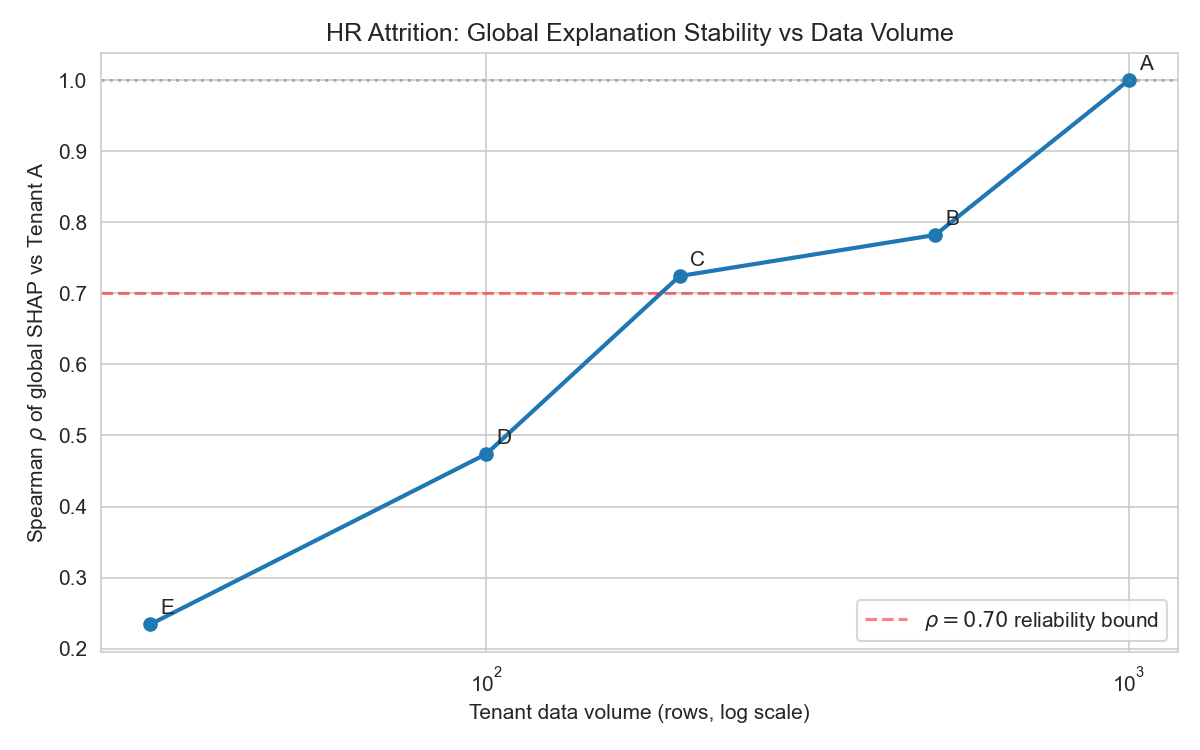
\includegraphics[width=0.75\linewidth]{hr_spearman_shap_degradation.png}
\caption{Per-tenant Spearman rank correlation of global SHAP
attributions against the Tenant~A baseline, Employee Attrition.}
\label{fig:hr-spearman}
\end{figure}

\begin{figure}[ht]
\centering
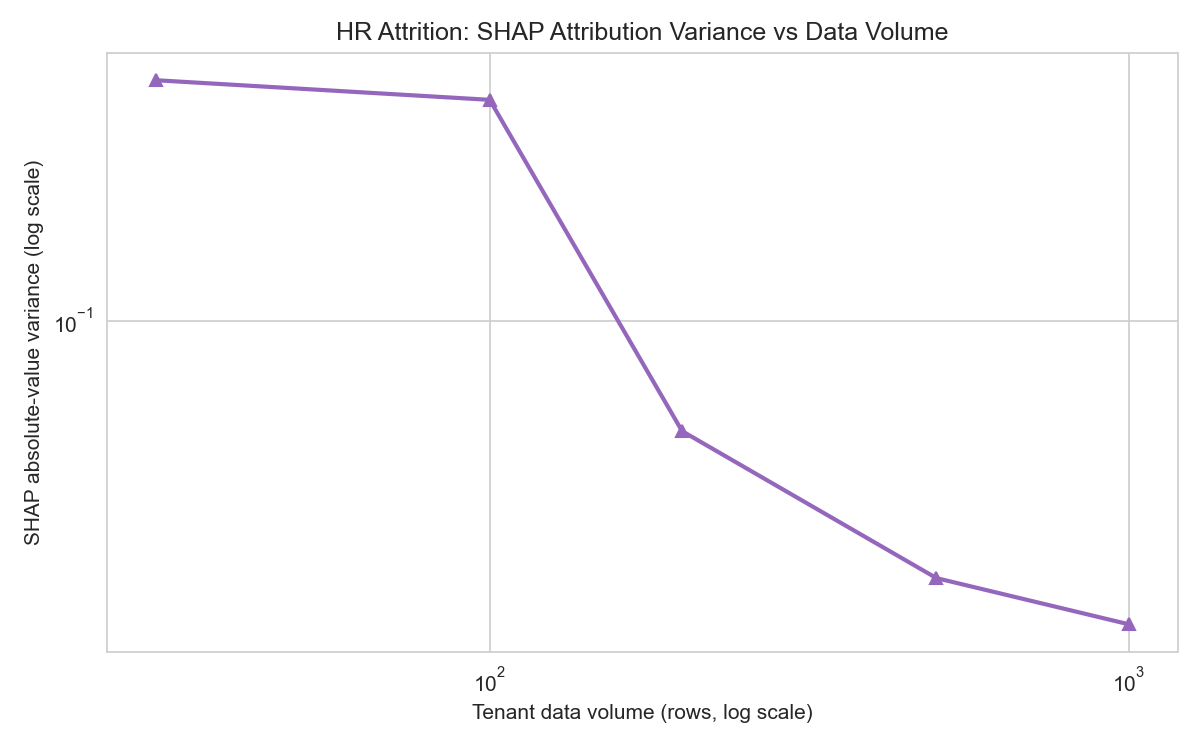
\includegraphics[width=0.75\linewidth]{hr_shap_variance_vs_volume.png}
\caption{Per-tenant SHAP absolute-value variance versus training
volume, Employee Attrition.}
\label{fig:hr-shap-variance}
\end{figure}

The qualitative regime change observed on the Late Delivery Risk task
replicates on Employee Attrition. Spearman rank correlation degrades
monotonically from $1.000$ to $0.234$, crossing the $\rho < 0.70$
boundary between Tenants~C and~D; SHAP absolute variance rises from
$0.025$ at Tenant~A to $0.299$ at Tenant~E---an $11.9\times$ expansion
concentrated between Tenants~C and~D, exactly where the rank-correlation
boundary is crossed. LIME top-5 Jaccard stability collapses monotonically
from $0.565$ at Tenant~A to below $0.20$ from Tenant~D onward. The
``grasping at straws'' degeneracy is again diagnostic at the cold-start
boundary: Tenant~E's SHAP attribution is concentrated on a single
feature (\texttt{MonthlyIncome}, attribution $= 3.671$) with zero
mean entropy, while AUC has collapsed to chance level ($0.500$). In
contrast to the Late Delivery Risk study---where cold-start AUC was
anomalously high---the HR predictive trajectory degrades together with
the explanation trajectory, so on this task predictive metrics
\emph{would} flag the cold-start regime; the methodological lesson is
not that predictive metrics are universally uninformative under
sparsity but that they are an \emph{unreliable safeguard} which on
some datasets happens to mislead exactly when an explanation-fidelity
safeguard is most needed.

\subsection{Lead Scoring (CRM Leads)}
\label{subsec:lead-scoring-replication}

The synthetic CRM Leads corpus contains $5{,}000$ pipeline records
with a binary \texttt{won}/\texttt{lost} target at $21.3\%$ positive
prevalence and $34$ post-encoding features. Personally identifying
fields (names, contact information, identifiers) and the
post-conversion \texttt{conversion\_date} field, which is populated
only on won leads and therefore constitutes target leakage by
construction, were excluded prior to training. The full-data
reference model achieved AUC-ROC $= 0.719$ and $F_1 = 0.114$.
Per-tenant results are reported in
Table~\ref{tab:lead-scoring-tiers}.

\begin{table}[ht]
\centering
\small
\caption{Cross-tier results, Lead Scoring (synthetic CRM Leads).}
\label{tab:lead-scoring-tiers}
\begin{tabular}{lrrrrrr}
\toprule
Tenant & $n$ & AUC & $F_1$ & $\rho$ vs A & $|\textnormal{SHAP}|$ var. & LIME Jacc. \\
\midrule
A (data-rich)   & $5{,}000$ & $0.702$ & $0.113$ & $1.000$ & $0.0307$ & $0.213$ \\
B (medium)      & $1{,}000$ & $0.733$ & $0.316$ & $0.408$ & $0.0271$ & $0.302$ \\
C (sparse)      & $300$     & $0.617$ & $0.267$ & $0.332$ & $0.0643$ & $0.387$ \\
D (very sparse) & $100$     & $0.547$ & $0.000$ & $0.372$ & $0.1251$ & $0.457$ \\
E (cold-start)  & $30$      & $0.200$ & $0.000$ & $0.493$ & $0.3439$ & $0.706$ \\
\bottomrule
\end{tabular}
\end{table}

\begin{figure}[ht]
\centering
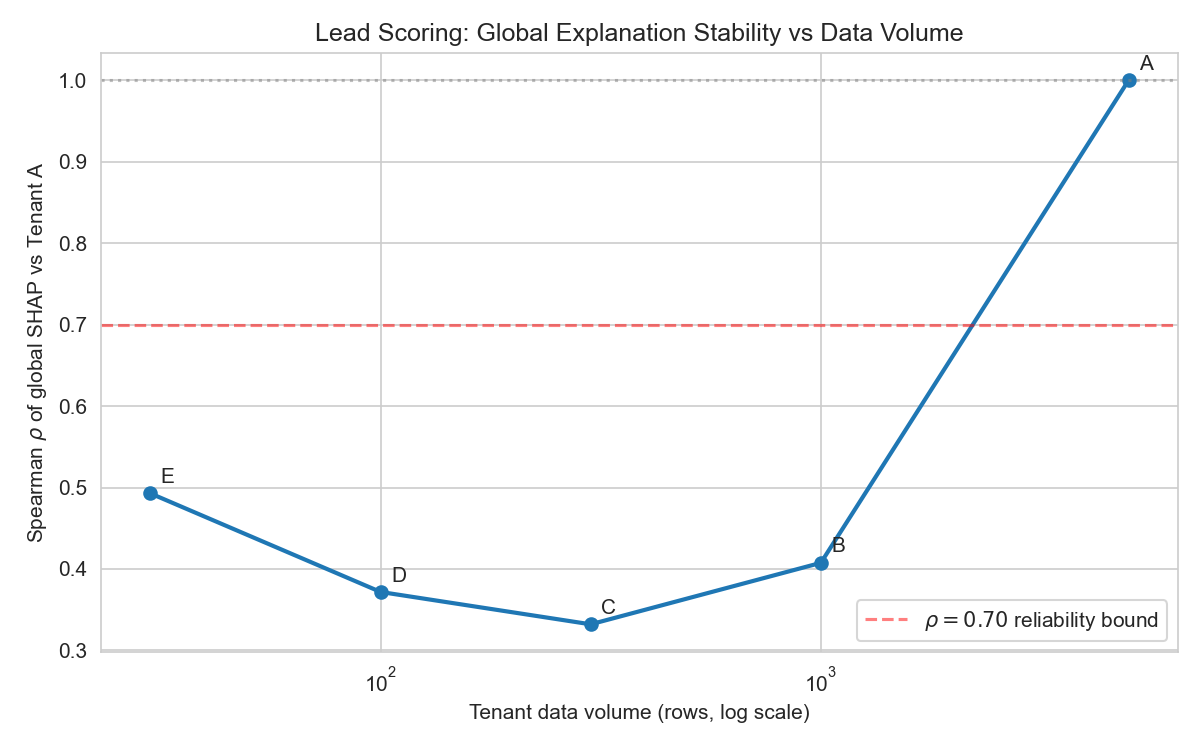
\includegraphics[width=0.75\linewidth]{lead_spearman_shap_degradation.png}
\caption{Per-tenant Spearman rank correlation of global SHAP
attributions against the Tenant~A baseline, Lead Scoring.}
\label{fig:lead-spearman}
\end{figure}

\begin{figure}[ht]
\centering
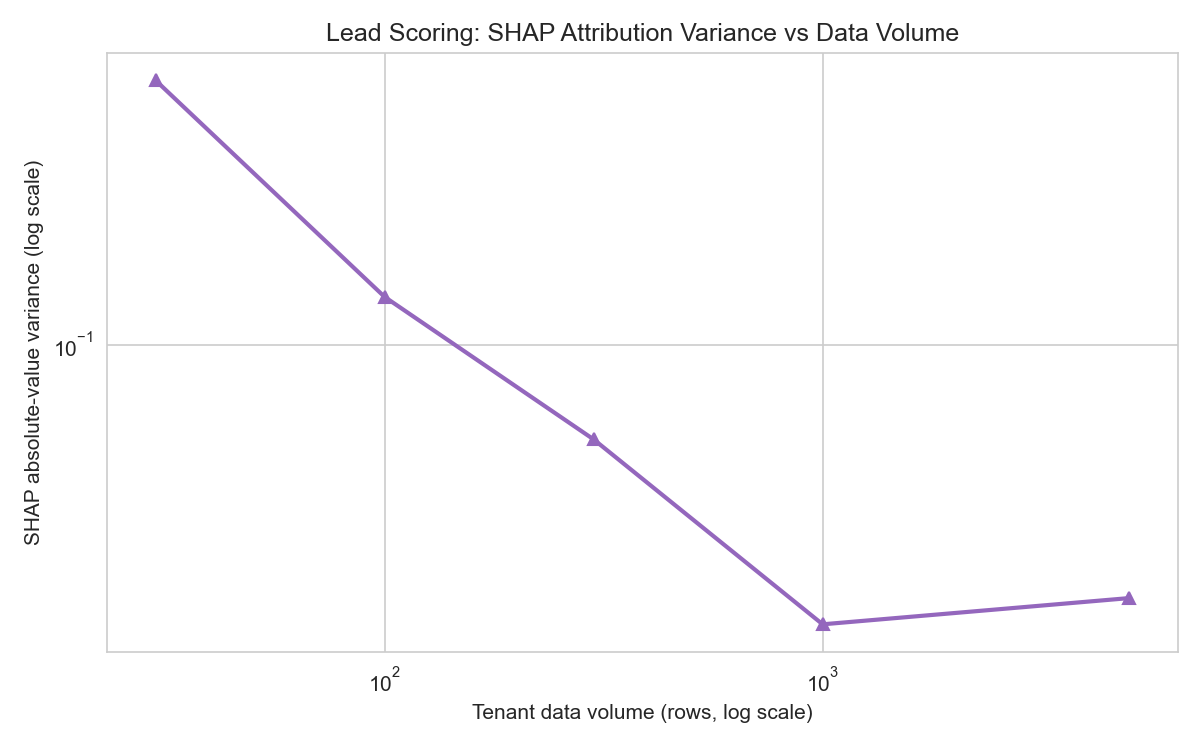
\includegraphics[width=0.75\linewidth]{lead_shap_variance_vs_volume.png}
\caption{Per-tenant SHAP absolute-value variance versus training
volume, Lead Scoring.}
\label{fig:lead-shap-variance}
\end{figure}

Lead Scoring confirms the structural finding while exposing two
methodologically important pathologies. First, SHAP absolute variance
again undergoes a $\approx 11\times$ expansion from Tenant~A to
Tenant~E ($0.031 \to 0.344$), with the expansion concentrated between
Tenants~C and~D, fully consistent with the cliff observed on the Late
Delivery Risk and Employee Attrition tasks. AUC degrades from $0.702$ at
Tenant~A through chance level at Tenant~D to an anti-predictive
$0.200$ at the cold-start tier, demonstrating that small-sample
volatility can flip the sign of the apparent decision rule entirely.
Second, the Lead Scoring task exhibits a feature-dominance regime in
which a single CRM-set field (\texttt{probability}) accounts for the
overwhelming share of SHAP attribution at Tenants~A--D, so the
Spearman trajectory enters its low-correlation regime as early as
Tenant~B and varies non-monotonically thereafter; this is itself an
ERP-realistic finding, because operationally configured features
of this kind are common in CRM pipelines and they amplify
sparsity-induced rank instability whenever the dominant feature's
attribution magnitude is itself perturbed by re-sampling. Third---and
counter-intuitively---LIME top-5 Jaccard stability \emph{rises} from
$0.213$ at Tenant~A to $0.706$ at Tenant~E, the inverse of the
trajectory observed on Late Delivery Risk and Employee Attrition. Inspection
of the per-tenant explanations shows that at the cold-start boundary
the model collapses into a near-univariate classifier that
deterministically returns the same one or two features for every
perturbation; the elevated Jaccard score therefore measures the
\emph{degeneracy} of the explainer rather than its trustworthiness.
This is the most operationally important methodological corollary of
the cross-task study: a single explanation-stability metric, read in
isolation, can be inverted by an extreme degeneracy regime, and an
explanation-fidelity safeguard must therefore concur over multiple
diagnostics---in particular Spearman rank correlation and SHAP
absolute variance---rather than rely on a single stability metric.

\subsection{Cross-Task Synthesis}
\label{subsec:cross-task-synthesis}

Across all three tasks the SHAP absolute-variance cliff replicates
with comparable magnitude ($226\times$, $11.9\times$ and $11.2\times$
A-to-E expansion for Late Delivery Risk, Employee Attrition and Lead Scoring
respectively) and the Spearman rank correlation against the data-rich
baseline crosses the $\rho < 0.70$ boundary in every task. The
predictive trajectory is task-dependent (anomalously high cold-start
AUC on Late Delivery Risk, chance-level on Employee Attrition,
anti-predictive on Lead Scoring), confirming that predictive metrics
cannot be relied upon to flag the explanation-fidelity collapse. The
absolute threshold $\tau$ at which the cliff occurs is also
task-dependent---on Employee Attrition it shifts to a smaller $n$
relative to Late Delivery Risk, plausibly reflecting the lower feature
dimensionality of the substrate, while on Lead Scoring the boundary
is masked by a configuration-feature dominance regime---but the
\emph{qualitative} architectural finding is invariant: post-hoc
explanation fidelity collapses through a regime change as training
volume falls, the collapse is not announced by predictive metrics,
and the safeguard must therefore be architectural. The
$\tau = 1{,}000$ threshold adopted for the
\texttt{COLD\_START\_INVOICE\_THRESHOLD} constant of the
\texttt{LatePaymentPredictor} is task-specific by design; the
cross-task replication justifies the broader
\emph{Maturity-Aware AI Routing} pattern, with per-task thresholds
to be calibrated empirically for each downstream ERP module.

\section{Threats to Validity}
\label{sec:threats}

\subsection{Internal Validity}
\label{subsec:internal-validity}

The five simulated tenants in this study were obtained by stratified slicing
of the underlying corpora (Olist Late Delivery Risk for the primary study,
supplemented by the IBM HR Analytics Employee Attrition corpus and the
synthetic CRM Leads corpus for the cross-task replication
in Section~\ref{sec:cross-task-replication}).
Although class prevalence and the global hold-out evaluation set were held
constant across tiers in order to isolate data volume as the manipulated
variable, the simulated tenants are not drawn from fundamentally different
business types or generative processes. Real-world multi-tenant ERPs may
exhibit additional inter-tenant variation---different industries, transaction
mixes, or customer geographies---that this simulation does not capture. The
findings should therefore be interpreted as identifying a \emph{necessary}
failure mode of post-hoc XAI under sparsity, not as having mapped its full
empirical surface.

\subsection{External Validity}
\label{subsec:external-validity}

The experiments are based on tabular ERP-style data; the explainers studied
(SHAP TreeExplainer, SHAP LinearExplainer, LIME tabular) are those most
commonly deployed in this setting. The cross-task replication reported in
Section~\ref{sec:cross-task-replication} demonstrates that the
explanation-fidelity cliff transfers across all three ERP-native tasks
committed to in the methodology, supporting the external validity of the
\emph{qualitative} regime change. Generalisation to unstructured-data
domains (text, image, multimodal) or to fundamentally different model
families (deep neural networks, recommendation systems) would require
additional empirical work. The \emph{qualitative} result---that post-hoc
explainers will produce confident outputs on top of degenerate models---is
theoretically expected to transfer, but the \emph{quantitative} threshold
($\tau = 1{,}000$) is task-specific and would
need to be re-derived per task and per model class, as the cross-task
study itself illustrates.

\subsection{Statistical Conclusion Validity}
\label{subsec:statistical-conclusion}

The small-sample volatility of the Tenant~E predictive metrics
($n = 50$, AUC $= 0.8889$, F1 $= 0.6667$) illustrates the inherent
fragility of point estimates computed on very small training partitions.
With only 50 training records the per-tenant model effectively reduces to
a near-univariate classifier (SHAP variance $= 5.04$,
\texttt{estimated\_delivery\_days} carrying an attribution $25\times$ the
next feature), and the apparent generalisation of that single feature to
the 19{,}292-row hold-out is one realisation of a high-variance estimator
rather than evidence of a stable predictive capability. The methodological
implication is exactly the converse of the leakage-prone version of this
argument: it is precisely because AUC \emph{is itself volatile and
occasionally flattering} at very small $n$ that the architectural
threshold in this thesis cannot be grounded in AUC and must be grounded
in the concurrence of the Spearman and SHAP-variance criteria. A future
robustness study should repeat the cold-start partition across multiple
seeds and report the empirical distribution of $\rho$ and SHAP variance,
but the qualitative finding---that explanation fidelity degrades through
a regime change in the absence of any predictive signal that could warn
the operator---is structurally invariant to seed choice.

\section{Chapter Summary}
\label{sec:results-summary}

This chapter has empirically established that, in a multi-tenant ERP
environment and under a strict leakage-avoidance regime, post-hoc
explanation fidelity collapses as tenant data volume decreases through a
regime change at approximately $n = 1{,}000$, while classical predictive
metrics neither track nor reveal that collapse. Spearman rank correlation
against the data-rich baseline falls monotonically from $1.0000$ to
$0.4485$, and SHAP absolute variance rises by more than two orders of
magnitude from $0.0224$ at Tenant~A to $5.0392$ at Tenant~E; meanwhile
AUC-ROC remains uniformly modest across tiers~A--D ($\approx 0.61$--$0.66$)
and anomalously \emph{rises} to $0.8889$ at the cold-start tier. The
simultaneous occurrence of an AUC of $0.8889$ and a top-feature SHAP
attribution of $4.77$ at Tenant~E operationalises the
\emph{Hallucinated Explanation Paradox} posited theoretically in
Chapter~\ref{ch:literature-review} in its sharpest form: the cold-start
model appears, by predictive metrics alone, to be the strongest in the
deployment, yet its explanation is rank-misaligned with the data-rich
baseline and concentrated on a single feature to a degree no business
interpretation can support. The empirical concurrence of the Spearman and
variance criteria at the $n = 1{,}000$ boundary justifies the adoption of
\texttt{COLD\_START\_INVOICE\_THRESHOLD = 1000} as the architectural gate
of the Maturity-Aware AI Routing pattern, whose implementation inside the
\texttt{LatePaymentPredictor} class structurally prevents cold-start
tenants from being shown local SHAP or LIME explanations that the
underlying data does not support---a safeguard whose necessity, in the
leakage-free regime, cannot be inferred from predictive metrics at all.
The cross-task replication on the IBM HR Analytics Employee Attrition
corpus and the synthetic CRM Leads corpus
(Section~\ref{sec:cross-task-replication}) confirms that the same
qualitative regime change occurs on the two further ERP-native
prediction tasks committed to in the methodology, supporting the
external validity of the architectural finding while making explicit
that the absolute threshold $\tau$ is task-specific and must be
re-derived per module.
The next chapter consolidates these findings into the conclusions and
recommendations of the thesis.
